% Figure s02f06_archetypes (Session 2): three two-dimensional dispersions and their densities of states.
% The image is rendered by figures/blender/s02f06_archetypes.py; the coordinates of the labels come from
% figures/blender/out/s02f06_archetypes_anchors.tex. Build with figures/blender/build_figure.sh s02f06_archetypes.
\documentclass[11pt,tikz,border=0pt]{standalone}
\usepackage[T1]{fontenc}
\usepackage{amsmath,amssymb,graphicx,bm}
\usepackage{xcolor}
\usetikzlibrary{arrows.meta,calc}
% The three label colors of the figures, with the same values as in src/figures_preamble.tex.
\definecolor{aqmaccent}{RGB}{31,78,121}
\definecolor{aqmbroken}{RGB}{168,42,34}
\definecolor{aqmmuted}{RGB}{125,125,125}

\newlength{\figw}\setlength{\figw}{15.6cm}   % the text width of the notes (A4, 2.7 cm margins)

\begin{document}
\begin{tikzpicture}[lbl/.style={font=\small, inner sep=1.5pt}, pnl/.style={font=\small\bfseries, inner sep=1.5pt}]
  \node[anchor=south west, inner sep=0pt] at (0,0)
    {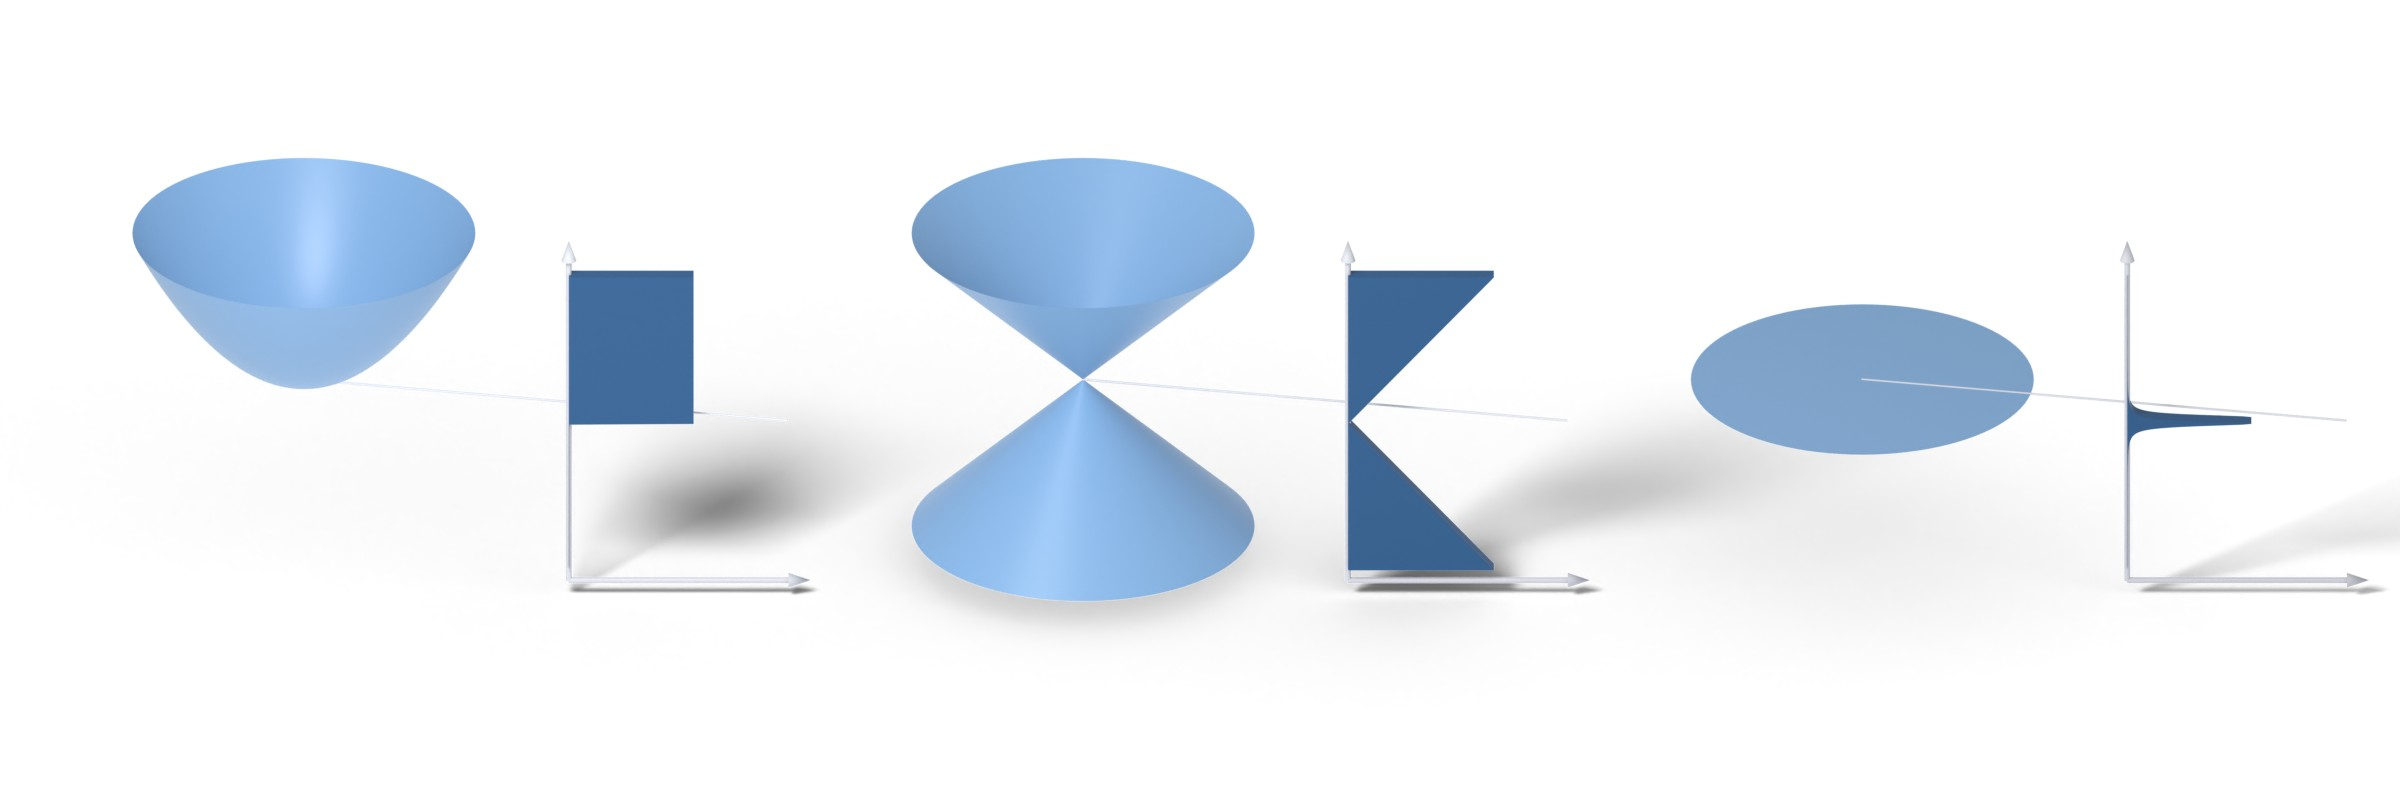
\includegraphics[width=\figw]{../blender/out/s02f06_archetypes.jpg}};
  %% written by figlib.py; x and y in units of the image width
\coordinate (aE) at (0.2370\figw,0.2330\figw);
\coordinate (ag) at (0.3377\figw,0.0916\figw);
\coordinate (aband) at (0.1266\figw,0.0652\figw);
\coordinate (azero) at (0.2370\figw,0.1581\figw);
\coordinate (bE) at (0.5617\figw,0.2330\figw);
\coordinate (bg) at (0.6623\figw,0.0916\figw);
\coordinate (bband) at (0.4513\figw,0.0652\figw);
\coordinate (bzero) at (0.5617\figw,0.1581\figw);
\coordinate (cE) at (0.8864\figw,0.2330\figw);
\coordinate (cg) at (0.9870\figw,0.0916\figw);
\coordinate (cband) at (0.7760\figw,0.0652\figw);
\coordinate (czero) at (0.8864\figw,0.1581\figw);

  \foreach \p/\t in {a/{parabolic band}, b/{Dirac cone}, c/{flat band}} {
    \node[lbl, anchor=south] at (\p E) {$\epsilon$};
    \node[lbl, anchor=south east] at (\p g) {$g$};
    \node[lbl, anchor=north] at (\p band) {\t};
  }
\end{tikzpicture}
\end{document}
